\documentclass[a4paper,11pt]{book}
\usepackage[spanish, activeacute]{babel}
\usepackage[utf8]{inputenc}
\usepackage{lmodern}
\usepackage[T1]{fontenc}
\usepackage{times}
\usepackage{graphicx}
\graphicspath{{fig/}}
\usepackage{multirow}
\usepackage{color}
\definecolor{gray97}{gray}{.97}
\definecolor{gray75}{gray}{.75}
\definecolor{gray45}{gray}{.45}
\usepackage[colorlinks=true, linkcolor=black, urlcolor=blue, filecolor=blue]{hyperref}
\usepackage{amsfonts}
\usepackage{anysize} 
\marginsize{3cm}{3cm}{2cm}{2cm}

\usepackage{listings}
\lstset{ frame=Ltb,
framerule=0pt,
aboveskip=0.5cm,
framextopmargin=3pt,
framexbottommargin=3pt,
framexleftmargin=0.4cm,
framesep=0pt,
rulesep=.4pt,
backgroundcolor=\color{gray97},
rulesepcolor=\color{black},
%
stringstyle=\ttfamily,
showstringspaces = false,
basicstyle=\small\ttfamily,
commentstyle=\color{gray45},
keywordstyle=\bfseries,
%
numbers=left,
numbersep=15pt,
numberstyle=\tiny,
numberfirstline = false,
breaklines=true,
%
tabsize=4
}

\newcommand\mytitleTFG{Ya mejoraremos el título}
\newcommand\myauthor{Autor 1}
\newcommand\myadvisor{José L. Risco Martín}
\newcommand\mydegree{Grado en Ingeniería Informática}
\newcommand\myyear{2020}
\newcommand\mycourse{2019/2020}

\title{\mytitleTFG}
\author{\myauthor}
\date{\today}
\makeindex

\begin{document}
\baselineskip 1.5em     % 2em doble espacio, 1em espacio sencillo.

%%% PORTADA %%%
\titlepage{}
\setlength{\unitlength}{1 cm} %Especificar unidad de trabajo

\begin{center}
\textbf{\LARGE \mytitleTFG}\\[1.25cm]
\LARGE{\myauthor}\\[1.25cm]
\textbf{{\LARGE Máster en Ingeniería Informática, Facultad de Informática, Universidad Complutense de Madrid}\\[0.5cm]}
\begin{figure}[!ht]
\begin{center}

\includegraphics[height=5cm,]{fig/logoucm.png}\\[0.5cm]
\end{center}
\end{figure}

{\LARGE Trabajo Fin de Máster}\\[0.5cm]
{\Large Junio de \myyear}\\[3cm]
\end{center}
\hfill \textbf{\Large Director:}\\

\hfill {\Large José Luis Risco Martín}


%%% ÍNDICE %%%
\tableofcontents

%%%Resumen y palabras clave %%%
\chapter*{Palabras clave}
\addcontentsline{toc}{chapter}{Palabras clave}
\markboth{Palabras clave}{Palabras clave}

\section*{Palabras clave en Español}
\begin{itemize}
\item Modelado y simulación
\item Sistemas de eventos discretos
\item Formalismo DEVS y xDEVS
\item Raspberry Pi
\item Módulos del kernel de Linux
\item Circuitos lógicos y secuenciales
\end{itemize}

\section*{Keywords in English}
\begin{itemize}
\item Modeling and simulation
\item Discrete events system
\item DEVS formalism and xDEVS
\item Raspberry Pi
\item Linux kernel Modules
\item Logic and sequential circuits
\end{itemize}

\chapter*{Resumen}
\addcontentsline{toc}{chapter}{Resumen}
\markboth{Resumen}{Resumen}

\section*{Título del trabajo}
Resumen en español de la propuesta.

\section*{Title in English}
Summary in english.

\chapter{Introducción, objetivos y plan de trabajo}
Capítulo 1

\section{Introducción}
Introducción

\section{Objetivos}
Objetivos

\section{Metodología y plan de trabajo}
Plan de trabajo

\section{Estructura del documento}
Estructura del documento
\chapter{Visión General}

\section{El formalismo DEVS}

\subsection{Introducción}
DEVS es un acrónimo de Discret Event System Specification \cite{Zeigler2000}. DEVS es un formalismo para el modelado y análisis de sistemas de eventos discretos. El término es ahora estándar en el campo de la simulación para referirse a un formalismo modular y jerárquico para modelar y analizar sistemas de diversos tipos. En particular, sistemas de eventos discretos, sistemas de ecuaciones diferenciales ó sistemas continuos y también sistemas híbridos continuos y discretos. En cualquiera de los casos, son sistemas de eventos cronometrados.
El formalismo DEVS fue creado por Bernard P. Zeigler, profesor emérito en la Universidad de Arizona, EE.UU.. DEVS fue presentado al público en su primer libro, Teoría de Modelado y Simulación, en el año  1976. DEVS se puede ver como una extensión del formalismo de la máquina de Moore, que es un autómata de estados finitos, donde las salidas están determinadas por el estado actual y no dependen de la entrada. De acuerdo a la teoría de DEVS, un sistema real se puede representar como un modelo construido en base a la experimentación que se quiera realizar y las condiciones de trabajo existentes. De esta forma, el modelo está restringido a la experimentación para la cual fue creado.
En el formalismo DEVS, un sistema está formado por subsistemas, los cuales se corresponden con modelos atómicos o modelos acoplados. Los acoplados están compuestos a su vez por otros modelos atómicos y/o acoplados. De esta forma, al disponer de sistemas complejos, es fácil probar los subsistemas individualmente.

Bajo un punto de vista general, un modelo DEVS está caracterizado por recibir entradas $X$, en relación con el estado con el que se encuentren $S$, generar eventos de salida $Y$, cada cierto tiempo.

\begin{figure}[!ht]
\begin{center}
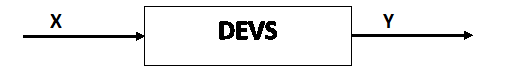
\includegraphics[height=2cm,]{Figura2_1.png}\\[0.5cm]
Figura 2.1: Representación del modelo DEVS
\end{center}
\end{figure}
\bigskip

\subsection{Descripción del formalismo DEVS}
DEVS define el comportamiento del sistema, así como la estructura del sistema. El comportamiento del sistema, en el formalismo DEVS es descrito utilizando eventos de entrada y salida, así como estados. La estructura del sistema se determina según la naturaleza del mismo.
En la Figura 2.2, como ejemplo intuitivo, se muestra el modelado en DEVS del juego del Ping-Pong.

\begin{figure}[!ht]
\begin{center}
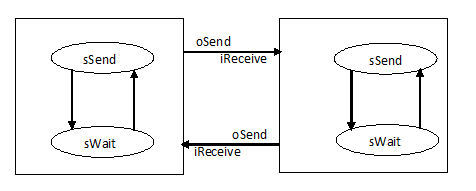
\includegraphics[height=5cm,]{Figura2_2.png}\\[0.5cm]
Figura 2.2: Modelado DEVS para el juego de Ping-Pong
\end{center}
\end{figure}

En el PingPong hay dos jugadores, A y B, y ambos están caracterizados por lo siguiente:
\begin{itemize}
\item Entrada: $iReceive$. Revela si el adversario ha lanzado la pelota y hará que se pase al estado sSend.
\end{itemize}
\begin{itemize}
\item Salida: $oSend$. Indica si el jugador ha lanzado la pelota (1) o aún no lo ha hecho (0).
\end{itemize}
\begin{itemize}
\item Estados: $sSend$ y $sWait$. Según las entradas y el tiempo transcurrido va cambiando de uno a otro.
\end{itemize}

En el formalismo DEVS clásico, DEVS Atómico captura el comportamiento del sistema, mientras que DEVS Acoplado describe la estructura del sistema.

\subsubsection{DEVS atómico}
Un modelo DEVS simple o atómico esta especificado bajo la 7-tupla:
\begin{equation}\label{eq:DevsAtomic}
M = \langle X,S,Y,\delta_{int},\delta_{ext},\lambda,\tau\rangle
\end{equation}

\noindent donde:

\begin{itemize}
\item $X$ : Es el conjunto de entrada.	
\item $S$ : Es el conjunto de estados. 
\item $Y$ : Es el conjunto de salida.
\item $\delta_{int}$ : $S\rightarrow S$, es la función de transición interna.
\item $\delta_{ext}$ : $Q\times X\rightarrow S$, es la función de transición externa, con
\begin{equation}\label{eq:FullState}
Q = \lbrace(s,t_e) | s\in S, t_e\in [0,\tau (s)]\rbrace
\end{equation}
\item $\lambda$ : $S\rightarrow Y$, es la función de salida.
\item $\tau$ : $S\rightarrow \mathbb{R}^{+}_{0}$, es la función que mide el tiempo.
\end{itemize}

\begin{figure}[!ht]
\begin{center}
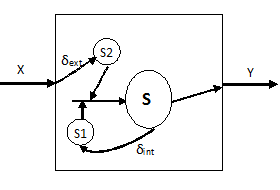
\includegraphics[height=6cm,]{Figura2_3.png}\\[0.5cm]
Figura 2.3: Modelo atómico DEVS
\end{center}
\end{figure}

La figura 2.3 muestra el comportamiento interno de un modelo DEVS atómico. Cada atómico tiene unas entradas $X$ y unas salidas $Y$ que van a permitirle comunicarse con otros modelos. La función de duración $\tau$ define el tiempo de vida del estado actual del modelo $S$. Los estado se actualizan al pasar el tiempo con la función de transición interna $\delta{int}$:$S{1}$->$S$. Al actualizarse el estado, se reflejan los cambios en las salidas $Y$ por medio de la función de salida $\lambda$. En cualquier momento, el modelo, puede recibir eventos de entrada que actualizarán el estado del modelo por medio de la función de transición externa $\delta{ext}$:$S{2}$->$S$, y reiniciarán el tiempo de vida del estado.
A continuación se muestra la descripción según el formalismo DEVS de los modelos atómicos $A$ y $B$ del juego de Ping-Pong, cuya representación gráfica se puede ver en la figura 2.4 y el diagrama temporal en la figura 2.5.

\begin{equation}\label{eq:PingPong1}
Jugador = \langle X,S,Y,\delta_{int},\delta_{ext},\lambda,\tau\rangle
\end{equation}

\noindent donde:

\begin{itemize}
\item $X$ = $\langle(in,{i}Receive)\rangle, con {i}Receive \in\langle{0,1}\rangle$
\item $S$ = $(phase,\sigma,{i}Receive), con phase \in\langle"{s}Wait","{s}Send"\rangle,\sigma \in {R}^{+}_{0}$
\item $Y$ = $\langle(out,{o}Send)\rangle, con {o}Send \in\langle{0,1}\rangle$
\item $\delta_{int}("{s}Wait","{s}Send")$ = $("{s}Wait",\inf,\phi)$
\item $\delta_{ext}("{s}Wait",\sigma,{i}Receive,t{e},(in,{i}Receive^{'}))$ = $("{s}Send",t{iReceive},{i}Receive^{'})$
\item $\lambda("{s}Send",\sigma,{i}Receive)$ = 1
\item $\lambda("{s}Wait",\sigma,{i}Receive)$ = 0
\end{itemize}

\begin{figure}[!ht]
\begin{center}
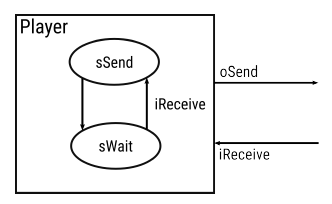
\includegraphics[height=5cm,]{Figura2_4.png}\\[0.5cm]
Figura 2.4: Modelo atómico DEVS de un jugador de Ping-Pong
\end{center}
\end{figure}

\begin{figure}[!ht]
\begin{center}
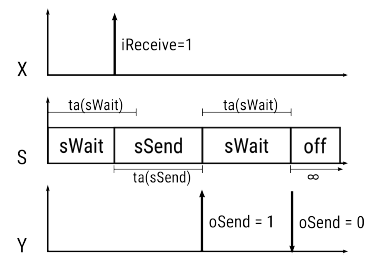
\includegraphics[height=5cm,]{Figura2_5.png}\\[0.5cm]
Figura 2.5: Diagrama de tiempo del modelo atómico DEVS de un jugador de Ping-Pong
\end{center}
\end{figure}

\subsubsection{DEVS acoplado}
El DEVS acoplado define qué subcomponentes pertenecen a él y cómo están conectados entre sí. Un modelo DEVS acoplado esta especificado bajo la 6-tupla:

\begin{equation}\label{eq:DevsAcoplado}
CM = \langle X,Y,C_{i},EIC,IC,EOC\rangle
\end{equation}

\noindent donde:

\begin{itemize}
\item $X$ : Es el conjunto de entrada.	
\item $Y$ : Es el conjunto de salida. 
\item $C_{i}$ : Es el conjunto de índices de componentes.
\item $EIC$ : Es el conjunto de componentes siendo cada $EIC$ un DEVS atómico.
\item $IC$ : Función de traslación de las salidas de $C_{i}$ a las entradas de $C_{j}$.
\item $EOC$ : Función de acoplamiento de las salidas de $C_{i}$ a las salidas del modelo acoplado.
\end{itemize}

El modelo acoplado DEVS está compuesto por modelos atómicos y/o acoplados cuyas entradas y salidas han sido interconectados entre ellos y el acoplado que los contiene. Cada modelo interno tiene un identificador $i$ y un conjunto de componentes $C{i}$. Las funciones de traslación \textit{EIC, IC y EOC} conectan respectivamente, las entradas del acoplado con las entradas de $C{i}$, las salidas de $C{i}$ con las entradas de $C{j}$ y las salidas de $C{i}$ con las salidas del acoplado.
Ya definido el modelo atómico del jugador del Ping-Pong, se describe a continuación, según el formalsmo DEVS, el modelo acoplado del juego, mostrado en la figura 2.2.

\begin{equation}\label{eq:DevsPingPong2}
PingPong = \langle X,Y,C{i},EIC,IC,EOC\rangle
\end{equation}

\noindent donde:

\begin{itemize}
\item $X$ = 0
\item $Y$ = 0 
\item $C{Jugador}$ = $\langle A,B\rangle$
\item $EIC$ = 0
\item $IC$ = $\langle (A.out,B.in),(B.out,A.in)\rangle$
\item $EOC$ = 0
\end{itemize}

\subsubsection{Simulación DEVS}
Los modelos DEVS pueden ser simulados de manera eficiente y sencilla. El algoritmos básico de simulación es el siguiente:

\begin{enumerate}
\item Encontrar el modelo atómico de $C{i}$ que, según su función $\tau$ y el tiempo transcurrido $t$, deba ser el próximo en ejecutar su $\delta{int}$.
\item Se adelanta $t$ hasta $t{n}$ el tiempo de la transición $\delta{int}$.
\item Se ejecutan las funciones $\lambda$ y $\delta{int}$ del modelo atómico de $C{i}$.
\item Tras ejecutar la función $\lambda$ se propagan las nuevas salidas $Y$ a todos los atómicos conectados con ellas y se ejecutan las funciones $\delta{ext}$ de los mismos.
\item Se vuelve al paso 1.
\end{enumerate}

Para la implementación de este algoritmo en un lenguaje de programación debe tenerse en cuenta cada modelo atómico tiene asociado un simulador DEVS y cada modelo acoplado un coordinador DEVS, como se puede ver en la figura 2.6.
\bigskip

\begin{figure}[!ht]
\begin{center}
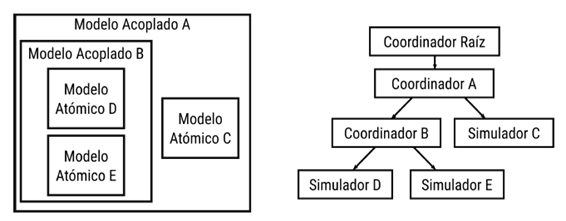
\includegraphics[height=5cm,]{Figura2_6.png}\\[0.5cm]
Figura 2.6: Estructura jerárquica de la simulación DEVS
\end{center}
\end{figure}

DEVS trata al modelo y al simulador como dos elementos diferentes. Cada componente tiene un protocolo de simulación y cada protocolo es impuesto por un proceso, el cual puede ser un coordinador o un simulador como podemos ver en la figura 2.7.
Primero se construye el modelo acoplado y se crea un coordinador junto con el modelo. A continuación el coordinador divide el modelo acoplado en componentes atómicos y/o acoplados. En el caso de que un componente fuera un modelo acoplado entonces su simulador debería ser un coordinador. Podemos decir que cada modelo atómico tiene su simulador propio y cada acoplado tiene un coordinador.

\begin{figure}[!ht]
\begin{center}
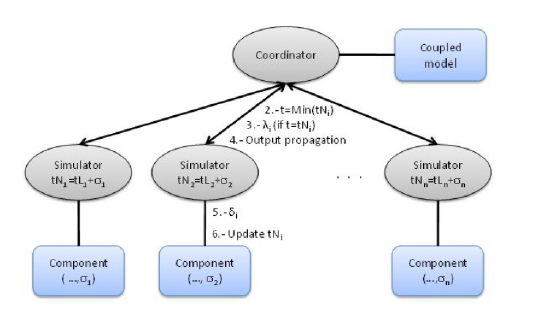
\includegraphics[height=8cm,]{Figura2_7.png}\\[0.5cm]
Figura 2.7: DEVS protocolo de simulación
\end{center}
\end{figure}

Una vez con el sistema construido, el coordinador raíz se encargará de encontrar el modelo atómico $M{d}$ que según su función ta() y el tiempo transcurrido, deba ser el próximo en ejecutar su función $\delta{int}$ (se ejecutará primero el que tenga un ta() menor). Después se le sumará al tiempo transcurrido el tiempo $t{n}$ de la transición $\delta{int}$ y se ejecutarán las funciones $\lambda$ y $\delta{int}$ de $M{d}$.
Tras ejecutar la función $\lambda$ se propagarán las nuevas salidas a todos los componentes conectados con ellas y se ejecutarán las funciones $\delta{ext}$ de los mismos. A continuación se limpiarán los puertos $X/Y$ y se volvería a buscar el atómico que le toca realizar su $\delta{int}$. Todo esto es un bucle que según los parámetros del usuario, simular durante un número de iteraciones, o por otro lados durante un tiempo específico.

Actualmente existen diversos proyectos que permiten desarrollar modelos DEVS y simularlos, por ejemplo:
\begin{itemize}
\item DEVSJAVA
\item DEVS/C++
\item PowerDEVS
\item xDEVS
\end{itemize}

Para este trabajo se ha elegido la plataforma xDEVS, desarrollado en el departamento de Arquitectura de Computadores y Automática de la Universidad Complutense de Madrid.  

\subsection{La plataforma xDEVS}
XDEVS es una plataforma de modelado y simulación DEVS implementada en Java, cuyo núcleo está disponible en https://github.com/jlrisco/xdevs. En su implementación se cubre la creación de modelos atómicos y acoplados, extendiendo a las clases respectivas, y cuenta con las clases necesarias para poder realizar una simulación completa. La simulación se realiza por medio de Coordinadores que pueden ejecutar en tiempo real o virtual.

\section{Simulación distribuida DEVS}
Las simulaciones distribuidas se utilizan principalmente para interoperar simuladores heterogéneos o modelos geográficamente distribuidos. Veremos algunas:

\subsection{Paralelo-DEVS}
Esta extensión desarrollada por el profesor Zeigler es proporcionar una técnica sencilla para la computación paralela, extensiones tradicionales utilizan técnicas en las que se distribuyen las ramas de la jerarquía de los modelos en los ordenadores. Un punto de sincronización es necesario realizar una prueba en la causalidad de los eventos. Las técnicas de sincronización se describen en técnicas optimistas, como Time Warp, y pesimista. Estas técnicas, aunque muy bien descrita, no se han aplicado por razones de servicios públicos en los modelos que utilizamos. Método DEVS paralelo utiliza un método simple de computación en paralelo usando un modelo de paralelización que hacen estallar cuando en una fecha en el calendario, todos los modelos de funciones de transición internas o externas se realizan en paralelo.
DEVS conjuntos paralelos de DEVS clásicos. Utilizamos DEVS clásicos con los puertos. 

\subsection{DEVS-Suite}
Es un simulador DEVS paralelo con soporte para automatizar el diseño de experimentos en combinación con modelos de animación, generar trayectorias de datos de tiempo superdensos en tiempo de ejecución, y tiempo de ejecución sincronizado del tiempo Junto con el componente jerárquico y la animación de mensajes de E/S. La versión 3.0.0 fue lanzada el 11 de abril de 2015.

\subsection{CD++}
CD++ es un programa destinado a la modelización y a la simulación de acontecimientos discretos. Las dos se organizan según el formalismo DEVS. CD++ puede funcionar en diferentes modos: en modo autónomo (soló un ordenador), en modo servidor, en modo tiempo real y en modo paralelo con un cluster Linux. CD++ se utiliza en línea de comandos. Sin embargo, existe una interfaz gráfica llamada CD++Builder que funciona como un plugin para Eclipse.

\subsection{xDEVS}
Una API de simulador DEVS escrita en Java. DEVS significa el formalismo de la especificación de eventos discretos. 

\subsection{PyDEVS}
PyDev es un tercero plug-in para Eclipse . Es un entorno de desarrollo integrado (IDE) que se utiliza para la programación en Python apoyo refactorización de código, gráfica depuración, análisis de código entre otras características.

\subsection{aDEVS}
Es un C ++ biblioteca para la construcción de simulaciones de eventos discretos. Adevs basado en el sistema Evento Especificación DEVS discreto y dinámico DEVS formalismos de modelado; es compatible con simulación de eventos discretos en paralelo y un sistema de tiempo de ejecución para OpenModelica. Adevs es desarrollado por Jim Nutaro.
Adevs es software libre y libera antes de la liberación 2.8 se distribuye bajo GNU LGPL 2.0. La versión 2.8 adevs es liberado bajo una licencia BSD.

\subsection{James II}
JAMES II le ayuda a desarrollar aplicaciones de modelado y simulación. Proporciona una base sólida de abstracciones, algoritmos, flujos de trabajo y herramientas. Los ejemplos de código para que te va: soporte para varios formalismos está disponible (por ejemplo, CA, atribuyen Pi Cálculo, ML-DEVS, o ML-reglas).
Simule varias replicaciones en paralelo, distribuya las ejecuciones entre los procesadores. Exploración de parámetros, optimización basada en simulación y controladores de experimentos personalizados. Selección automática de algoritmos y reconfiguración adaptativa en tiempo de ejecución.

\subsection{DEVSim++}
Dev-C ++ es un libre de todas las funciones de entorno de desarrollo integrado (IDE) se distribuye bajo la Licencia Pública General de GNU para la programación en C y C ++. Está escrito en Delphi.Se incluye el MinGW o TDM-CCG puerto de 64 bits de la CCG como su compilador. Dev-C ++ también se puede utilizar en combinación con Cygwin o cualquier otro compilador basado en GCC.Dev-C ++ es generalmente considerado un sólo para programas Windows, pero hay intentos de crear una versión de Linux: archivos de cabecera y delimitadores de ruta se puede conmutar entre plataformas.

\subsection{RESTful-CD ++}
El primer middleware de simulación distribuido basado en REST (Representational State Transfer) Servicios web. El middleware RESTful-CD ++ permite la interacción entre componentes de simulación heterogéneos desarrollados independientemente Con mucha flexibilidad y sencillez. REST tiene el potencial de avanzar la simulación distribuida de vanguardia hacia
Plug-and-play o interoperabilidad automática/semiautomática. Esto debido a su enfoque ligero oculta el software de implementación interno, mediante el uso de la interfaz universal uniforme y la descripción de la conectividad semántica en forma de mensajes, por lo general XML. En contraste, otros enfoques exponen funcionalidades en RPCs heterogéneos que a menudo reflejan la implementación interna y describir la semántica en forma de parámetros de procedimiento. 

\section{Simulación en la nube}
En el mercado actual existen diversos servicios para la realización de la simulación en la nube, aquí vamos a mencionar algunas de ellas:

\subsection{AWS}
Amazon Web Services es una colección de servicios de computación en la nube también llamados servicios web, que en conjunto forman una plataforma de computación en la nube, ofrecidas a través de Internet por Amazon.com. Es usado en aplicaciones populares como Dropbox, Foursquare, HootSuite. Es una de las ofertas internacionales más importantes de la computación en la nube y compite directamente contra servicios como Microsoft Azure y Google Cloud Platform. Es considerado como un pionero en este campo.
AWS está situado en 11 Regiones geográficas: EE.UU. Este (Norte de Virginia), EE.UU. Oeste (Norte de California), EE.UU. Oeste (Oregón), AWS GovCloud (EE.UU.), Sao Paulo (Brasil), Irlanda, Singapur, Tokio y Sydney. También hay un "GovCloud" en los EE.UU. proporcionado para los clientes del Gobierno de EE.UU.. Cada región está totalmente contenida dentro de un solo país y todos sus datos y servicios permanecen dentro de la región designada.
Cada región tiene múltiples "zonas de disponibilidad", que son los diferentes centros de datos que proporcionan servicios de AWS. Las zonas de disponibilidad están aisladas unas de otras para evitar la propagación de cortes entre las zonas. Varios servicios operan a través de zonas de disponibilidad por ejemplo, S3, DynamoDB, mientras que otros pueden estar configurados para reproducirse a través de zonas para extender la demanda y evitar el tiempo de inactividad de los fallos.

\subsection{Google Cloud Platform}
Google Cloud, es una plataforma que ha reunido todas las aplicaciones de desarrollo web que Google estaba ofreciendo por separado. Es utilizada para crear ciertos tipos de soluciones a través de la tecnología almacenada en la nube y permite por ejemplo destacar la rapidez y la escalabilidad de su infraestructura en las aplicaciones del buscador.
Google Cloud se refiere al espacio virtual a través del cual se puede realizar una serie de tareas que antes requerían hardware o software para lograr, pero en lugar de esto utilizas la nube de Google como tu única fuente de acceso, almacenamiento y gestión de datos.
Google ofrece una variedad de servicios basados en la nube. Google Cloud Print permite imprimir desde la web, el escritorio o dispositivo móvil sin la necesidad de un sistema operativo en particular o controladores. En su lugar, envías el documento a cualquier impresora conectada a la nube. Google también ofrece espacio en la nube para desarrolladores de bases de datos SQL para crear aplicaciones y para los usuarios de Microsoft Office que desean editar colaborativamente documentos de Word, PowerPoint y Excel, sin necesidad de software.
Provee también de resultados de búsqueda en milisegundos. Posee espacio de almacenamiento para más de 400 millones de usuarios del Gmail. La red global utilizada por Google Cloud Platform está abastecida por fibra óptica y conecta con todos los rincones del planeta. Usar esta plataforma significa tener acceso a todas las innovaciones de Google.

\subsection{Microsoft Azure}
Microsoft Azure anteriormente Windows Azure y Azure Services Platform es una distribución Linux ofrecida como servicio y alojada en los Data Centers de Microsoft. Anunciada en el Professional Developers Conference de Microsoft (PDC) del 2008 en su versión beta, pasó a ser un producto comercial el 1 de enero de 2010. Windows Azure es una plataforma general que tiene diferentes servicios para aplicaciones, desde servicios que alojan aplicaciones en alguno de los centros de procesamiento de datos de Microsoft para que se ejecute sobre su infraestructura (Cloud Computing) hasta servicios de comunicación segura y federación entre aplicaciones. En el reporte de Gartner Magic Quadrant más reciente, Azure fue uno de solo dos vendedores el otro siendo Amazon Web Services otorgado el título de Líderes.

\subsection{Citrix OpenCloud}
Citrix OpenCloud permite a las empresas crear nubes híbridas, y a los proveedores de servicios ofrecer soluciones de nube capaces de atender las cargas de trabajo empresariales. Una plataforma de tecnología rica y abierta, que ofrece funciones de virtualización, conexión en red y entrega de aplicaciones, junto a innovaciones en la federación de las redes y los dominios de identidad de las empresas y sus proveedores, haciendo posible para los departamentos de TI y los proveedores de servicios la creación y la gestión de entornos de nube seguros y con múltiples ocupantes, capaces de atender cargas de trabajo corporativas.

\subsection{HP Cloud}
HP Cloud era un conjunto de computación en la nube servicios disponibles por Hewlett-Packard que ofrecían nube pública, nube privada, nube híbrida, lograron nube privada, y otros servicios en la nube. Fue la combinación de la unidad anterior de HP Converged Nube negocio y HP Cloud Services, que es el OpenStack nube pública basada en la tecnología. Es utilizado por las organizaciones empresariales para que puedan combinar los servicios de nube pública con sus propios recursos internos de TI para crear nubes híbridas, o una mezcla de diferentes computación en la nube entornos compuestos de nubes públicas y privadas.

\subsection{IBM Cloud Computing}
IBM Cloud Computing es un conjunto de computación en la nube de servicios de negocio que ofrece la empresa de tecnología de la información de IBM. IBM Cloud incluye la infraestructura como servicio (IaaS), el software como servicio (SaaS) y plataforma como servicio (PaaS) ofrecido a través de modelos de prestación de nubes públicas, privadas e híbridas, además de los componentes que integran esas nubes.
IBM ofrece tres plataformas de hardware de computación en la nube. Estas plataformas ofrecen soporte incorporado para la virtualización. Para la virtualización de IBM ofrece IBM Websphere soluciones de infraestructura de aplicaciones que soportan los modelos de programación y estándares abiertos para la virtualización.
La capa de gestión del marco nube de IBM incluye IBM Tivoli middleware. Herramientas de administración proporcionan capacidades para regular las imágenes con automatizada de aprovisionamiento y de aprovisionamiento, control de los establecimientos y el uso del medidor mientras que el seguimiento y la asignación de los costos de facturación. La última capa de la estructura proporciona herramientas de carga de trabajo integrados. Las cargas de trabajo de computación en la nube son servicios o instancias de código que se puede ejecutar para satisfacer las necesidades específicas del negocio. IBM ofrece herramientas para la nube basada en la colaboración, el desarrollo y prueba, la aplicación desarrollo, análisis, integración de negocio a negocio, y la seguridad.

\subsection{OpenStack}
OpenStack es un proyecto de computación en la nube para proporcionar una infraestructura como servicio (IaaS).Es un software libre y de código abierto distribuido bajo los términos de la licencia Apache. El proyecto está gestionado por la Fundación OpenStack, una persona jurídica sin fines de lucro creada en septiembre de 2012 para promover el software OpenStack y su comunidad.
Más de 200 empresas se unieron al proyecto entre las que destacan AMD, Avaya, Brocade Communications Systems, Canonical, Cisco, Dell, Ericsson, Groupe Bull, HP, IBM, InkTank, Intel, NEC, Rackspace Hosting, Red Hat, SUSE Linux, VMware y Yahoo!.La tecnología consiste en una serie de proyectos relacionados entre sí que controlan estanques de control de procesamiento, almacenamiento y recursos de red a través de un centro de datos, todos administrados a través de un panel de control que permite a los administradores controlar mientras potencia a sus usuarios proveyendo los recursos a través de una interfaz web. La comunidad OpenStack colabora en torno a un ciclo de lanzamiento con hitos de desarrollo de frecuencia semestral.7 Durante la fase de planificación de cada lanzamiento, la comunidad se reúne para la Cumbre de Diseño OpenStack para facilitar sesiones de trabajo para desarrolladores y armar planes a futuro.

\subsection{Apache CloudStack}
CloudStack es un código abierto de computación en la nube de software para la creación, gestión y despliegue de servicios en la nube de infraestructura . Utiliza existentes hipervisores como KVM, VMware vSphere, y XenServer/XCP para la virtualización. Además de su propia API, CloudStack también es compatible con la API de Amazon Web Services (AWS) y de la Computación en la nube interfaz abierta desde el Open Grid Forum.
La instalación de producción mínima consiste en una máquina que ejecuta CloudStack Management Server y otra máquina para actuar como infraestructura de la nube, en este caso, una infraestructura muy simple que consiste en un host que ejecuta el software del hipervisor. En su despliegue más pequeño, una sola máquina puede actuar como el servidor de administración y el anfitrión hipervisor utilizando el hipervisor KVM. Múltiples servidores de administración se pueden configurar para la redundancia y balanceo de carga, todos apuntando a una base de datos común MySQL.

\chapter{Automatización DEVS utilizando Docker}

\section{Docker}

Docker es un proyecto de código abierto que automatiza el despliegue de aplicaciones dentro de contenedores de software, proporcionando una capa adicional de abstracción y automatización de Virtualización a nivel de sistema operativo en Linux. Docker utiliza características de aislamiento de recursos del kernel de Linux, tales como cgroups y espacios de nombres (namespaces) para permitir que "contenedores" independientes se ejecuten dentro de una sola instancia de Linux, evitando la sobrecarga de iniciar y mantener máquinas virtuales.

El soporte del kernel de Linux para los espacios de nombres aísla de vista, en su mayoría, una aplicación del entorno operativo, incluyendo árboles de proceso, red, ID de usuario y sistemas de archivos montados, mientras que los cgroups del kernel proporcionan aislamiento de recursos, incluyendo la CPU, la memoria, el bloque de E/S y de la red. Desde la versión 0.9, Docker incluye la biblioteca libcontainer como su propia manera de utilizar directamente las facilidades de virtualización que ofrece el kernel de Linux, además de utilizar las interfaces abstraídas de virtualización mediante libvirt, LXC (Linux Containers) y systemd-nspawn.

De acuerdo con la firma analista de la industria 451 Research, "Docker es una herramienta que puede empaquetar una aplicación y sus dependencias en un contenedor virtual que se puede ejecutar en cualquier servidor Linux. Esto ayuda a permitir la flexibilidad y portabilidad en donde la aplicación se puede ejecutar, ya sea en las instalaciones físicas, la nube pública, nube privada, etc.
%%% Bibliografía y Autorización %%%
\bibliographystyle{alpha}
\bibliography{bibliography}

\chapter*{Agradecimientos}
\addcontentsline{toc}{chapter}{Agradecimientos}
\markboth{Agradecimientos}{Agradecimientos}

Agradecimientos.
%% AUTORIZACIÓN %%
\chapter*{Autorización de difusión}
\addcontentsline{toc}{chapter}{Autorización de difusión}
\markboth{Autorización de difusión}{Autorización de difusión}
\section*{Autorización para la difusión del Trabajo Fin de Máster y su depósito en el Repositorio Institucional E-Prints Complutense}
{
\setlength{\parindent}{0cm}
El/la abajo firmante, matriculado/a en el Máster en Ingeniería Informática de la Facultad de Informática, autoriza a la Universidad Complutense de Madrid (UCM) a difundir y utilizar con fines académicos, no comerciales y mencionando expresamente a su autor el presente Trabajo Fin de Máster: ``\mytitleTFG'', realizado durante el curso académico \mycourse bajo la dirección de \myadvisor en el Departamento de Arquitectura de Computadores y Automática, y a la Biblioteca de la UCM a depositarlo en el Archivo Institucional E-Prints Complutense con el objeto de incrementar la difusión, uso e impacto del trabajo en internet y garantizar su preservación y acceso a largo plazo.

\bigskip
\bigskip
\bigskip
\bigskip
\bigskip
\bigskip
\bigskip
\bigskip

\hfill Madrid, a XX de junio de \myyear\\[1.5cm]

\hfill Fdo.: \myauthor
}


\end{document}
